\documentclass[border=8pt]{standalone}
\usepackage{tikz}
\usetikzlibrary{arrows.meta, positioning, fit}
\usepackage{helvet}
\usepackage[none]{hyphenat}
\usetikzlibrary{calc}
\renewcommand{\familydefault}{\sfdefault}

\definecolor{ink}{HTML}{202124}
\definecolor{muted}{HTML}{5F6368}
\definecolor{line}{HTML}{AAB0B6}
\definecolor{band}{HTML}{F7F8F9}
\definecolor{blue}{HTML}{2F6FA3}
\definecolor{bluesoft}{HTML}{EAF2F8}
\definecolor{green}{HTML}{168A55}
\definecolor{greensoft}{HTML}{E5F4EC}
\definecolor{orange}{HTML}{B56A18}
\definecolor{orangesoft}{HTML}{FFF1DF}

\tikzset{
  nodebase/.style={font=\sffamily\scriptsize, text=ink},
  band/.style={draw=line!65, fill=band, rounded corners=3pt},
  data/.style={nodebase, draw=blue, fill=bluesoft, rounded corners=2pt,
    align=center, minimum height=0.62cm, text width=3.5cm, inner sep=4pt},
  process/.style={nodebase, draw=ink!50, fill=white, rounded corners=2pt,
    align=center, minimum height=0.62cm, text width=3.5cm, inner sep=4pt},
  core/.style={nodebase, draw=green, fill=greensoft, rounded corners=2pt,
    align=center, minimum height=0.62cm, text width=3.5cm, inner sep=4pt},
  service/.style={font=\sffamily\scriptsize, text=orange!90!black,
    align=center, text width=1.65cm, inner sep=2pt},
  audit/.style={nodebase, draw=ink!45, fill=white, rounded corners=2pt,
    align=center, minimum height=0.60cm, text width=2.55cm, inner sep=3pt},
  final/.style={audit, draw=green, fill=greensoft},
  arrow/.style={-{Latex[length=1.8mm]}, draw=ink!70, line width=0.6pt},
  external/.style={-{Latex[length=1.8mm]}, draw=orange!90!black, dashed, line width=0.55pt},
  auditarrow/.style={-{Latex[length=1.8mm]}, draw=green!75!black, line width=0.65pt},
  label/.style={font=\sffamily\bfseries\scriptsize, text=muted},
  note/.style={font=\sffamily\scriptsize, text=muted, align=center}
}

\begin{document}
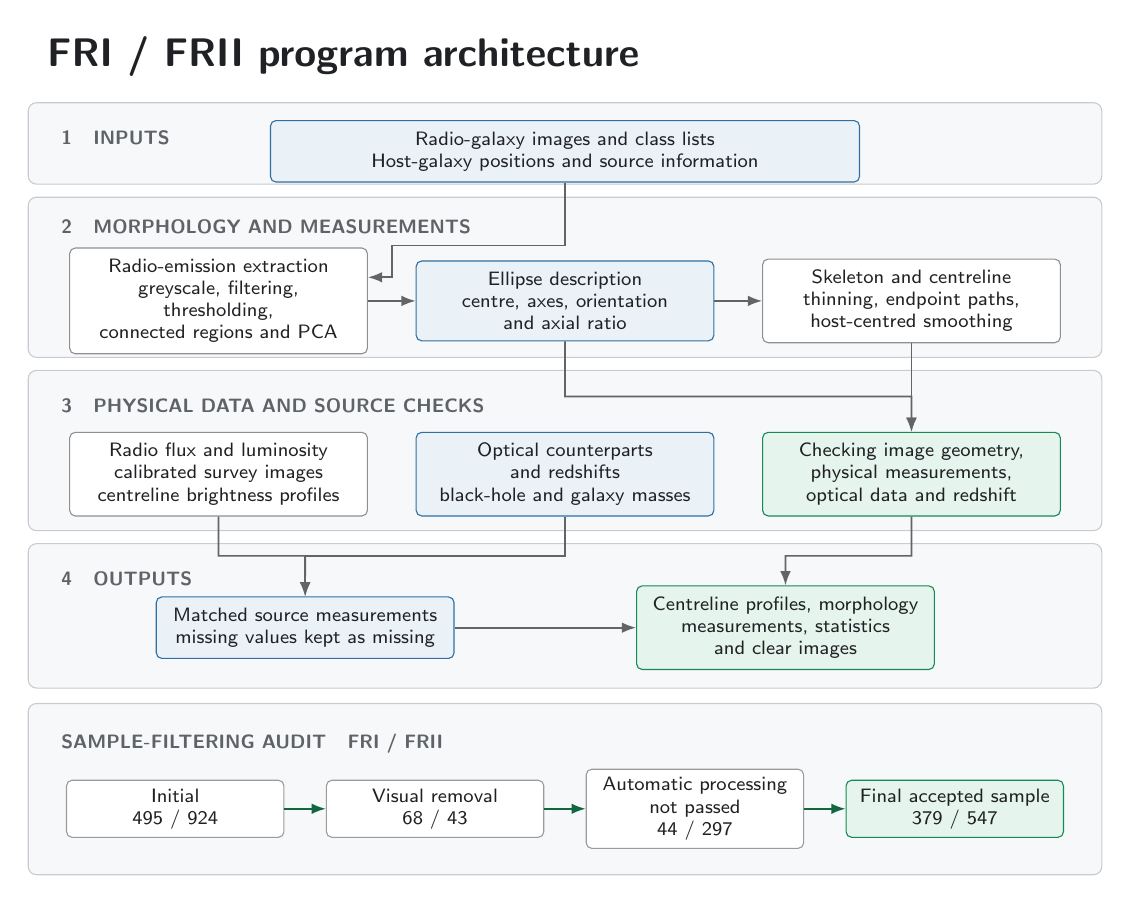
\begin{tikzpicture}[x=1cm,y=1cm]

\node[font=\sffamily\bfseries\Large, text=ink, anchor=west] at (0,10.45)
  {FRI / FRII program architecture};
\node[font=\sffamily\scriptsize, text=muted, anchor=west] at (0,10.10)
  {};

% Inputs
\node[band, fit={(0,8.95) (13.40,9.75)}] {};
\node[label, anchor=north west] at (0.18,9.63) {1\quad INPUTS};
\node[data, text width=7.2cm] (input) at (6.70,9.25)
  {Radio-galaxy images and class lists\\
   Host-galaxy positions and source information};

% Morphology and measurements
\node[band, fit={(0,6.75) (13.40,8.55)}] {};
\node[label, anchor=north west] at (0.18,8.50) {2\quad MORPHOLOGY AND MEASUREMENTS};
\node[process] (morph) at (2.30,7.35)
  {Radio-emission extraction\\greyscale, filtering, thresholding,\\connected regions and PCA};
\node[data] (geometry) at (6.70,7.35)
  {Ellipse description\\centre, axes, orientation\\and axial ratio};
\node[process] (fits) at (11.10,7.35)
  {Skeleton and centreline\\thinning, endpoint paths,\\host-centred smoothing};

% Physical data and quality control
\node[band, fit={(0,4.55) (13.40,6.35)}] {};
\node[label, anchor=north west] at (0.18,6.23) {3\quad PHYSICAL DATA AND SOURCE CHECKS};
\node[process] (optical) at (2.30,5.15)
  {Radio flux and luminosity\\calibrated survey images\\centreline brightness profiles};
\node[data] (mass) at (6.70,5.15)
  {Optical counterparts and redshifts\\black-hole and galaxy masses};
\node[core] (qc) at (11.10,5.15)
  {Checking image geometry, physical measurements,\\optical data and redshift};

% Outputs
\node[band, fit={(0,2.55) (13.40,4.15)}] {};
\node[label, anchor=north west] at (0.18,4.03) {4\quad OUTPUTS};
\node[data] (table) at (3.40,3.20)
  {Matched source measurements\\missing values kept as missing};
\node[core] (results) at (9.50,3.20)
  {Centreline profiles, morphology\\measurements, statistics and clear images};

% Main flow
\draw[arrow] (input.south) -- ++(0,-0.8) -- ++(-2.2,0) -- ++(0,-0.4) |- ($(morph.east)+(0, 0.3)$);
\draw[arrow] (morph) -- (geometry);
\draw[arrow] (geometry) -- (fits);
\draw[arrow] (fits.south) -- (qc.north);
\draw[arrow] (optical.south) -- ++(0,-0.5)  -- ++(1.1,0) -- (table.north);
\draw[arrow] (mass.south) -- ++(0,-0.5)  -- ++(-3.3,0) -- (table.north);
\draw[arrow] (table) -- (results);
\draw[arrow] (qc.south) -- ++(0,-0.5)  -- ++(-1.6,0) -- (results.north);

% Cross-stage dependency
\draw[arrow] (geometry.south) -- ++(0,-0.7)  -- ++(4.4,0) -- (qc.north);

% Sample audit
\node[band, fit={(0,0.18) (13.40,2.12)}] {};
\node[label, anchor=north west] at (0.18,1.98) {SAMPLE-FILTERING AUDIT\quad FRI / FRII};
\node[audit] (a0) at (1.75,0.9) {Initial\\495 / 924};
\node[audit] (a1) at (5.05,0.9) {Visual removal\\68 / 43};
\node[audit] (a2) at (8.35,0.9) {Automatic processing not passed\\44 / 297};
\node[final] (a3) at (11.65,0.9) {Final accepted sample\\379 / 547};
\draw[auditarrow] (a0) -- (a1);
\draw[auditarrow] (a1) -- (a2);
\draw[auditarrow] (a2) -- (a3);
\node[note, text width=12.2cm, anchor=north west] at (0.35,0.55)
  {};

\end{tikzpicture}
\end{document}
